 \documentclass[t,14pt]{beamer}
 %
 % Packages pour le français
 \usepackage[T1]{fontenc} 
 \usepackage[utf8]{inputenc}
 \usepackage[frenchb]{babel}
 %
 % pour un pdf lisible à l'écran
 % il y a d'autres choix possibles 
 \usepackage{pslatex}
\usetheme{Singapore}
  \usecolortheme{rose}
  \setbeamertemplate{blocks}[rounded][shadow=true]

\title{\textbf{\textit{Extraction et Analyse d'Images}}}
\subtitle{PED}
\author{\scriptsize{Manson Tomy\\
		Mestreau Nicolas\\
		Ridel Fabien\\
		Wen Jun\\
		\vspace{10mm}
		Encadrant : \\
		Laviole Jérémy\\
		}}
\institute{\tiny Université de Bordeaux 1}



\begin{document}

\frame{\titlepage}

%% part 1 - Jun
\section[Presentation]{Presentation}
\AtBeginSection[]{
\begin{frame}{Table of contents}
\small \tableofcontents[currentsection, hideothersubsections]
\end{frame}
}

\begin{frame}{Presentation}
\begin{center}
Un sujet proposé par Jérémy Laviole.
\vspace{2mm}
\end{center}
\end {frame}

%% part 2 - Fabien
\section[Pré-traitement]{Pretraitement}
\vspace{5mm}
\begin{frame}{Filtres}
\vspace{5mm}
\begin{itemize}[<+->]
\item Adaptation Tracker to Saliency descriptors (Saliency maps)
\item Integration tools in a unique software
\end{itemize}
\end{frame}

%% part 3 - Nicolas
\section[Détection de Pictogrammes]{Template Detector}
\begin{frame}{Objectif}
\vspace{5mm}
\begin{itemize}
\item Développer un logiciel qui détecte des pictogrammes dans un flux vidéo.
\item Utilisation de templates représentant les pictogrammes.
\vspace{5mm}
\begin{center}
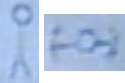
\includegraphics[scale=0.66]{images/templates.png}
\end{center}
\end{itemize}
\end{frame}

\begin{frame}{Méthode utilisée}
\vspace{5mm}
\begin{itemize}
\item Template Matching
\item Principe : 
\begin{center}
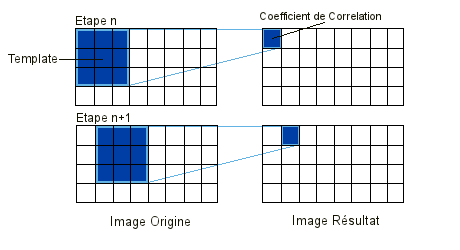
\includegraphics[scale=0.66]{images/templateMatching.png}
\end{center}
\end{itemize}
\end{frame}
			
\begin{frame}{Problème rencontré}
\vspace{5mm}
\begin{itemize}
\item \texttt{cvMatchTemplate} -> Carte de corrélation
\item Récupération du meilleur résultat
\item Difficulté pour déterminer un seuil d'acceptation
\end{itemize}
\end{frame}	

\begin{frame}{Résultats obtenus}
\vspace{5mm}
\begin{center}
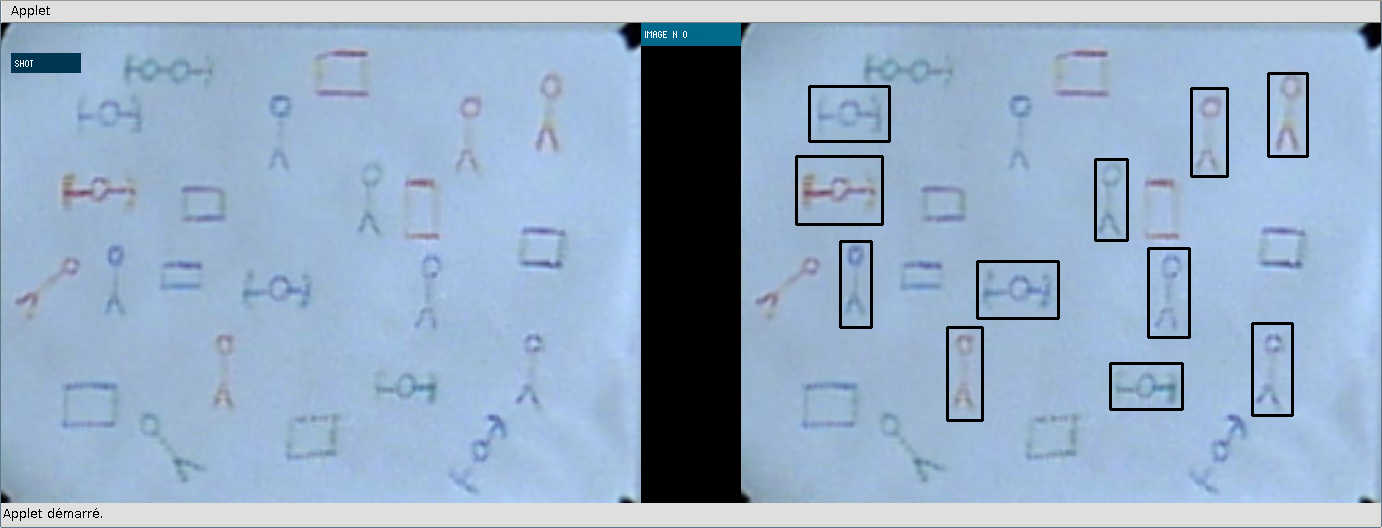
\includegraphics[width=\textwidth]{images/capture1.png}
\end{center}
\end{frame}

\begin{frame}{Résultats obtenus}
\vspace{5mm}
\begin{center}
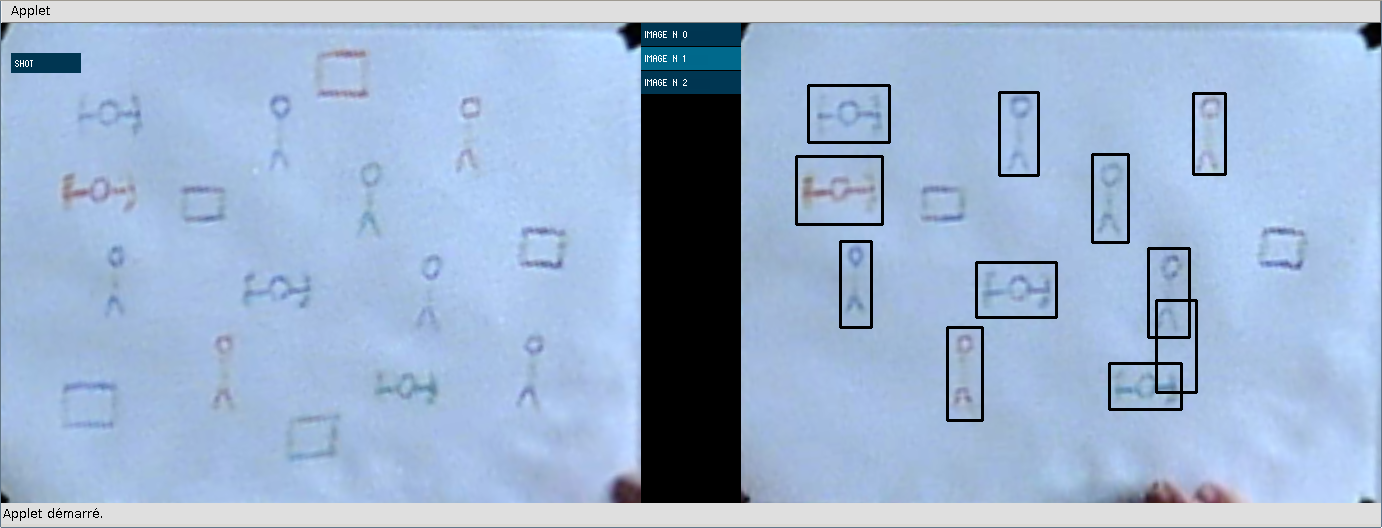
\includegraphics[width=\textwidth]{images/capture2.png}
\end{center}
\end{frame}

\begin{frame}{Méthode alternative}
\vspace{5mm}
\begin{itemize}
\item SURF
\item Intérêt : Non affecté par rotation et mise à l'échelle 
\item Problème : Qualité vidéo trop basse -> Trop peu de marqueurs détectés
\end{itemize}
\end{frame}
	
%% part 4 - Tomy
\section[Extraction de nouveautés]{Feature Extractor}
\begin{frame}{Objectif}
\vspace{5mm}
\begin{itemize}
\item Développer un logiciel qui permet de voir l'évolution d'un dessin.
\vspace{5mm}
\begin{center}
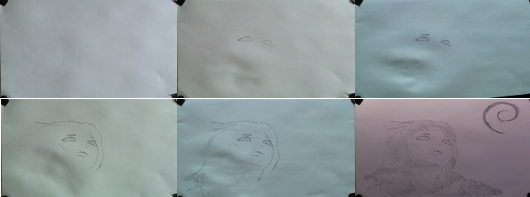
\includegraphics[scale=0.5]{images/evo/evo.png}
\end{center}
\end{itemize}
\end{frame}

\begin{frame}{Tâtonnement}
\begin{block}{}
Dans un premier temps nous avons fait une simple différences d'images.
\end{block}
\begin{center}
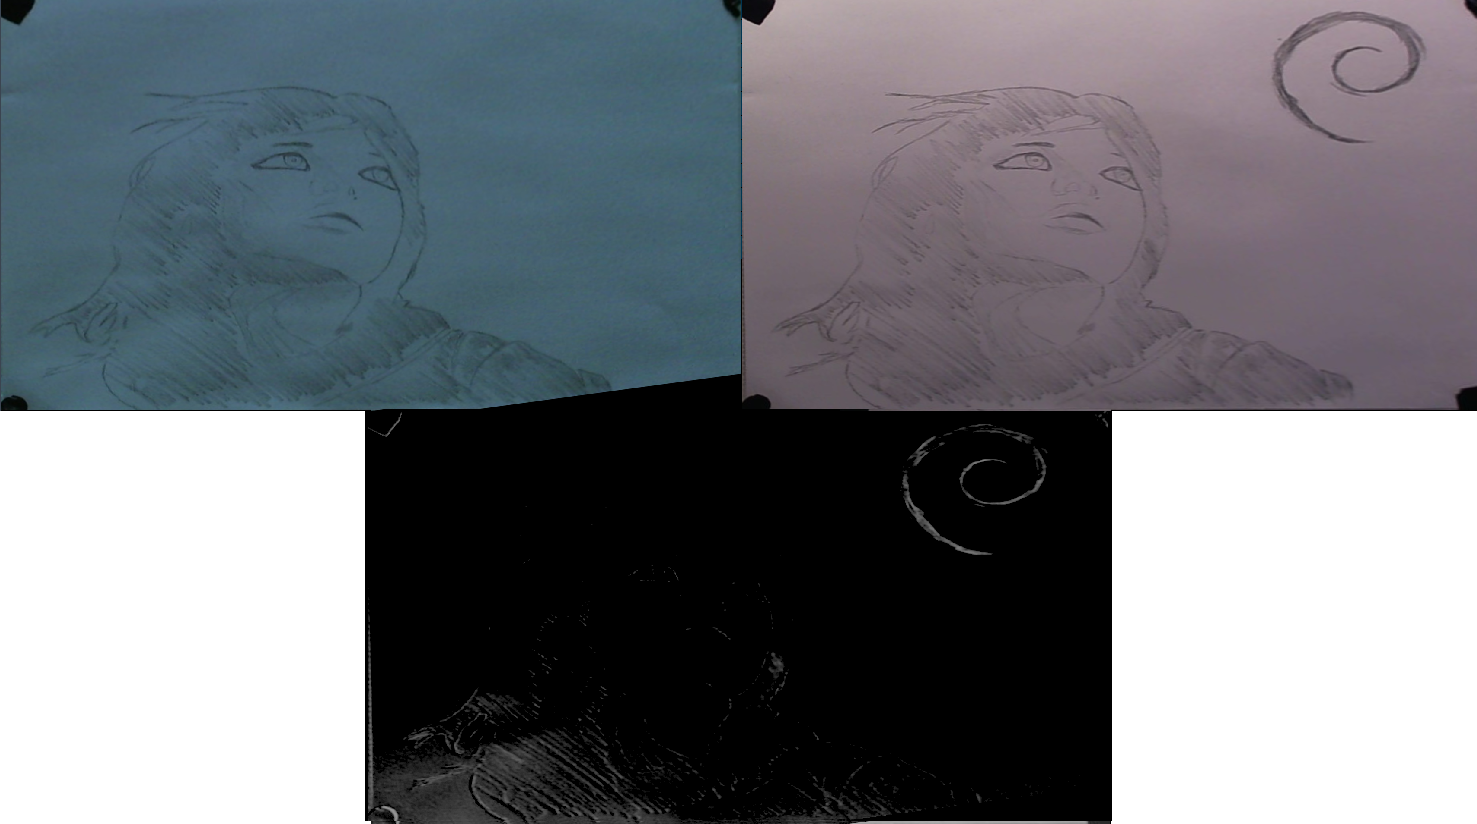
\includegraphics[width=\textwidth]{images/evo/diff.png}
\end{center} 
\end{frame}

\begin{frame}{Tâtonnement}
\begin{block}{}
Dans un premier temps nous avons fait une simple différences d'images.
\end{block}
\vspace{5mm}
\begin{itemize}
\item Problème : Impossible d'extraire les nouveautés
\item Solution : \'Etape de pré-traitement
\end{itemize}
\end{frame}

\begin{frame}{Pré-traitement}
\vspace{5mm}
\begin{block}{}
Les images que nous avons présentent des défauts.
\end{block}

\begin{itemize}
\item Coloration : 
	\begin{itemize}
	\item Le dessin est un processus long
	\item Rend l'analyse plus difficile
	\item Nécessité d'une balance des blancs
	\end{itemize}
\item Haute qualité :
	\begin{itemize}
	\item Rend l'analyse plus facile
	\item Augmente le temps d'analyse
	\item Algorithme efficace nécessaire
	\end{itemize}
\end{itemize}
\end{frame}

\begin{frame}{Méthode utilisée}
\vspace{5mm}
\begin{block}{}
\textbf{Idée :} extraction d'un masque de nouveautés
\end{block}
\begin{itemize}
\item Binarisation des images
\item Différence des images obtenues
\end{itemize}
\end{frame}

\begin{frame}{Résultats obtenus}
\vspace{5mm}
\begin{center}
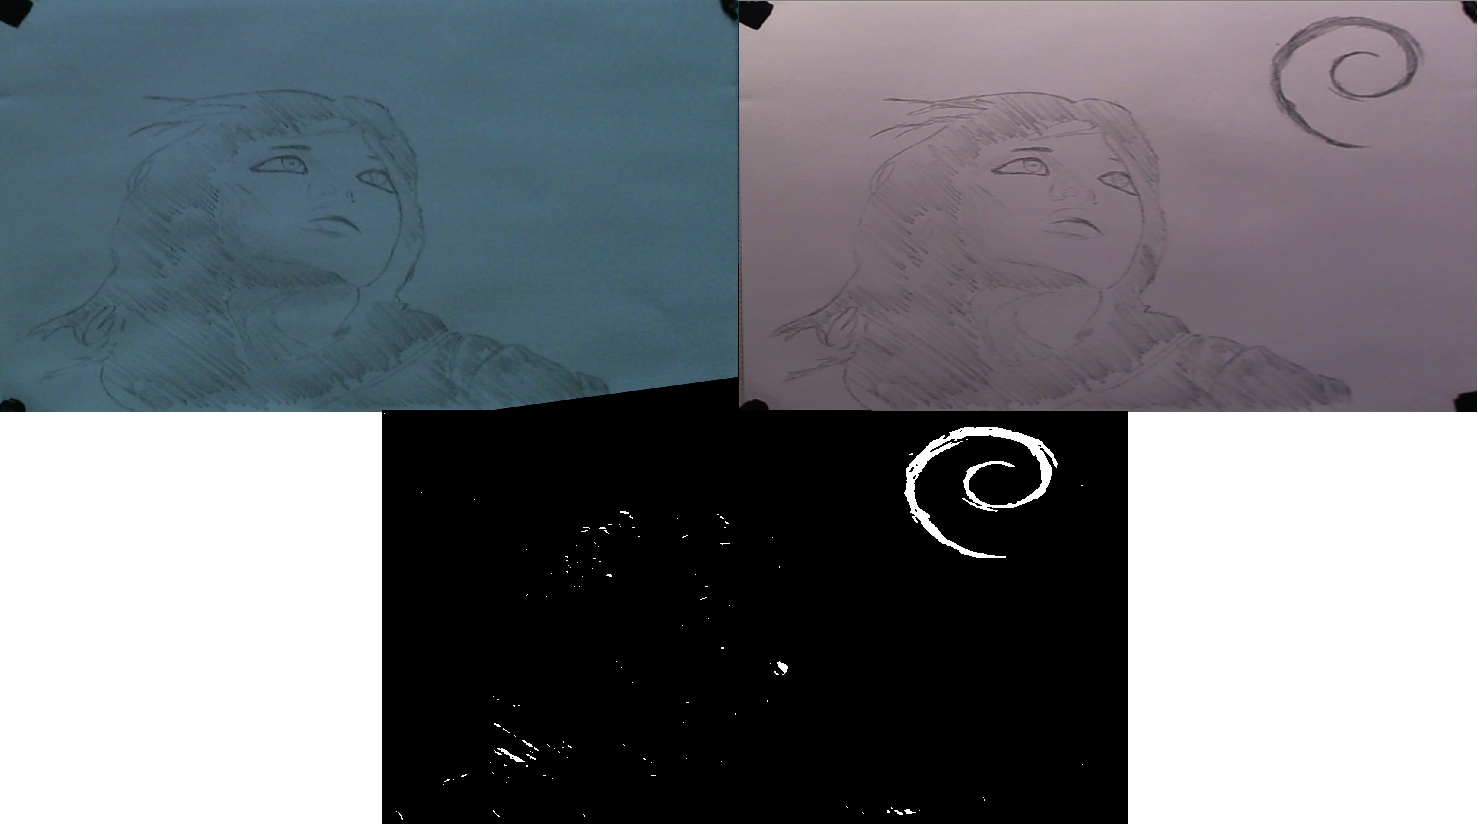
\includegraphics[width=\textwidth]{images/evo/masque.png}
\end{center}
\end{frame}


\begin{frame}{Résultats obtenus}
\vspace{5mm}
\begin{center}
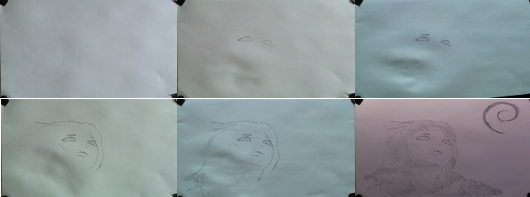
\includegraphics[width=\textwidth]{images/evo/evo.png}
\end{center}
\end{frame}
\begin{frame}{Résultats obtenus}
\vspace{5mm}
\begin{center}
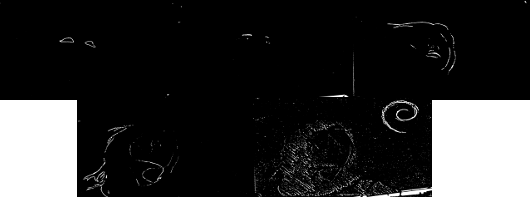
\includegraphics[width=\textwidth]{images/evo/evomasque.png}
\end{center}
\end{frame}
			
\begin{frame}{Problème rencontré}
\vspace{5mm}
\begin{block}{}
Il est difficile de supprimer totalement le bruit sur le masque
\end{block}
\begin{itemize}
\item Différence de recalage
\item Le dessinateur redessine par dessus
\end{itemize}
\end{frame}	

	
\section[Conclusion]{Conclusion}
	\begin{frame}{Conclusion}
		\vspace*{5mm}
		\begin{itemize}
		\end{itemize}
	\end{frame}

\end{document}
